\documentclass{article}
\usepackage{graphicx}
\usepackage[dvipsnames,table]{xcolor}
\usepackage[utf8]{inputenc}
\usepackage{siunitx}
\usepackage[american,siunitx]{circuitikz}
\usepackage{amsmath}
\usepackage{svg}
\usepackage{booktabs}
\usepackage{float}
\usepackage{xparse, xfp}
\usepackage{multirow}
\usepackage{tikz}
\usepackage{karnaugh-map}
\usepackage{pdfpages}
\usepackage{hyperref}
\hypersetup{
    colorlinks=true,
    linkcolor=blue,
    filecolor=magenta,      
    urlcolor=cyan,
}
\usetikzlibrary{calc}
%\usepackage[landscape]{geometry}
\renewcommand{\thesubsection}{\thesection.\alph{subsection}}
\newcommand{\equal}{=}
\newcommand{\greyrule}{\arrayrulecolor{black!30}\midrule\arrayrulecolor{black}}
\makeatletter
\newcommand\currcoor{\the\tikz@lastxsaved,\the\tikz@lastysaved}
\makeatother
\newcolumntype{:}{@{\hskip\tabcolsep\color{black!30}\vrule\hskip\tabcolsep}}

\ExplSyntaxOn
\NewExpandableDocumentCommand \groupify { O{\,\allowbreak} m m }
  { \jakob_groupify:nnn {#1} {#2} {#3} }
\cs_new:Npn \jakob_groupify:nnn #1 #2 #3
  { \__jakob_groupify_loop:nnw { 1 } {#2} #3 \q_recursion_tail {#1} \q_recursion_stop }
\cs_new:Npn \__jakob_groupify_loop:nnw #1 #2 #3
  {
    \quark_if_recursion_tail_stop:n {#3}
    \exp_not:n {#3}
    \int_compare:nNnTF {#1} = {#2}
      { \__jakob_groupify_sep:n }
      { \exp_args:Nf \__jakob_groupify_loop:nnw { \int_eval:n { #1+1 } } }
          {#2}
  }
\cs_new:Npn \__jakob_groupify_sep:n #1 #2 \q_recursion_tail #3
  {
    \tl_if_empty:nF {#2} { \exp_not:n {#3} }
    \__jakob_groupify_loop:nnw { 1 } {#1}
    #2 \q_recursion_tail {#3}
  }
\ExplSyntaxOff

\title{ECE 3301\\Introduction to Microcontrollers\\\,\\Assignment 4}
\author{Choi Tim Antony Yung}
\begin{document}
\maketitle

\thispagestyle{empty}
\setcounter{page}{0}

\newpage

\section{(30) Use MPLAB to write an asemply program to multipy two numbers (11111001) and (11111001). Then save the product in file reisters 0x50 and 0x51. Return a snapshot of your code, the SFR memory view showing the register used to store the multiplication, the file register view showing the product value.}
\begin{figure}[H]
  \centering
  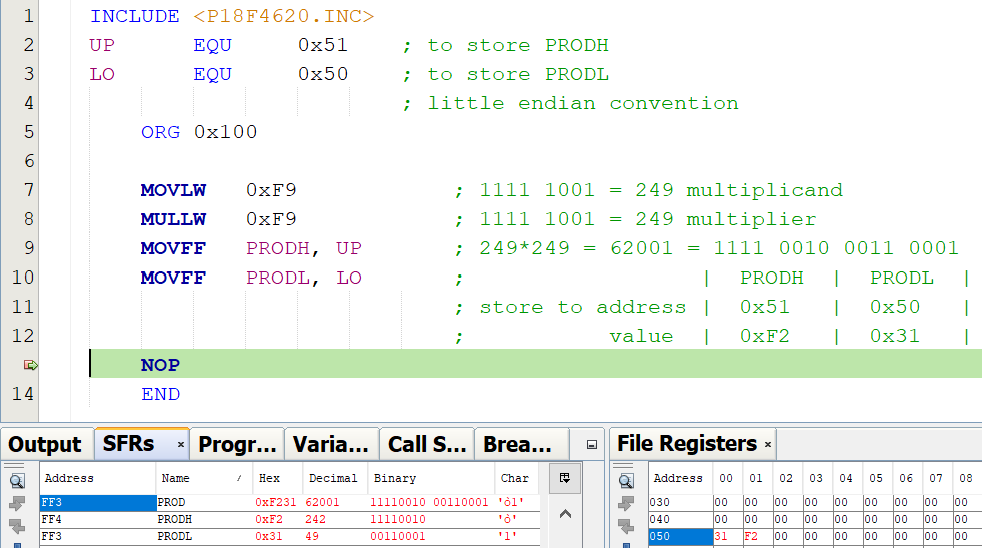
\includegraphics[width=\textwidth]{ECE3301_Assignment4.png}
  \caption{A snapshot of assmebly code to multiply the two number and the SFR memory annd file register view of the microcontroller after multiplication}
\end{figure}

\newpage

\section{(20) Use a table to show the differences between the program memory and data memory sizes, no of bits PC used to address the PM, max number of instructions, and FSR size, for the PIC18F family and the PIC18F4321 microcontroller.}

\begin{tabular}{r|p{4.5cm}p{3.7cm}}
  \toprule
  &PIC18F Family&PIC18F4321\\
  \midrule
            Program Memory size & $2^{21}\times8$ bits = Up to  2 MBytes &   8 KBytes                                                      \\
               Data Memory size & $2^{12}\times8$ bits = Up to  4 KBytes & 512 Bytes                                                       \\
  \# of bits used to address PM &                        Up to 21 Bits   &  13 Bits                                                        \\
  \midrule
     max number of instructions & $\frac{2\text{ MBytes memory}}{2\text{ Bytes instruction}}\newline=2^{20}=\text{Up to }1048576$ & $\frac{8\text{ KBytes memory}}{2\text{ Bytes instruction}}=4096$ \\
  \midrule
                       FSR size & \multicolumn{2}{c}{three 16-bit registers (FSR0, FSR1, FSR2)}\\
                                & \multicolumn{2}{c}{divided into 6 8-bit registers:}\\
                                & \multicolumn{2}{c}{FSR0H, FSR0L, FSR1H, FSR1L, FSR2H, FSR2L}\\
  \bottomrule
\end{tabular}

\newpage

\section{(20) Show the Configuration of the PIC18F4321 to operate on 2MHZ using a stable internal oscillator, enter the idle mode when it sleeps, no primary oscillator. Write the configuration value using both C and assembly language.}

\begin{tabular}{p{1.015cm}p{1.015cm}p{1.015cm}p{1.015cm}p{1.015cm}p{1.015cm}p{1.015cm}p{1.015cm}}
  7&6&5&4&3&2&1&0\\
\end{tabular}\\
\begin{tabular}{|p{1cm}|p{1cm}|p{1cm}|p{1cm}|p{1cm}|p{1cm}|p{1cm}|p{1cm}|}
  \hline
  1&1&0&1&0&1&1&x\\
  \hline
\end{tabular}\\
\begin{tabular}{p{1cm}p{1cm}p{1cm}p{1cm}p{1cm}p{1cm}p{1cm}p{1cm}}
  IDLEN&IRCF2&IRCF1&IRCF0&OSTS&IOFS&SCS1&SCS0\\
\end{tabular}\\
\newline
According to page 31 of \href{http://ww1.microchip.com/downloads/en/DeviceDoc/39689b.pdf}{the PIC18F4321 Datasheet}:\\
IDLEN = 1 : Device enters an Idle mode when a SLEEP instruction is executed\\
IRCF2:IRCF0 = 101 : 2 MHz\\
OSTS = 0: Oscillator Start-up Timer (OST) time-out is running; primary oscillator is not ready\\
IOFS = 1: INTOSC frequency is stable\\
SCS1:SCS0 = 1x: Internal oscillator block\\
\newline
Therefore, we can apply the above mentioned configuration by moving 0xD6 or 0xD7 to OSCCON.\\ 
\newline
Assembly:\\
MOVLW 0xD6\\
MOVWF OSCCON\\
\newline
C:\\
OSCCON = 0xD7

\newpage

\section{(15) How many fuctions are multiplexed on PIC18F4321 Pin 33 (PDIP package). Explain what each of these fuctions used for?}
According to page 18 of \href{http://ww1.microchip.com/downloads/en/DeviceDoc/39689b.pdf}{the PIC18F4321 Datasheet}:\\
Four functions are multiplexed on PIC18F4321 Pin 33 (PDIP package):\\
\newline
RB0: Digital I/O\\
INT0: External interrupt 0\\
FLT0: PWM Fault input for Enhanced CCP1\\
AN12: Analog input 12

\newpage

\section{(15) Use the PIC18 insteruction set pdf file on blackboard to find the machine code of the POP and the PUSH instructions, what is the size of the instruction? Also find the ASCII code of both instructions}

According to the PIC18 instruction set pdf file on blackboard:\\
\newline
Machine code of POP:\\
0000 0000 0000 0110 in binary, or 0x0006\\
\newline
Machine code of PUSH:\\
0000 0000 0000 0101 in binary, or 0x0005\\

The size of both instructions are 16 bits.\\
\newline
According to \href{https://en.wikipedia.org/wiki/ASCII}{the Wikipedia page of ASCII}, assuming all capital letter:\\
\newline
ASCII of POP:\\
0x504F50, or 0101 0000 0100 1111 0101 0000 in binary\\
\newline
ASCII of PUSH:\\
0x50555348, or 0101 0000 0101 0101 0101 0011 0100 1000 in binary\\
\end{document}
